%% ANGRYBIRDS AI FRAMEWORK ARCHITECTURE DOCUMENT
%%
%% FILENAME:    architecture.tex
%% AUTHOR:      Stephen Gould <sgould@stanford.edu>
%%

\documentclass[10pt,a4paper]{article}
\usepackage{amssymb,amsmath,latexsym}

\usepackage{fullpage}
\usepackage{amsfonts}
\usepackage{graphicx}
\usepackage[authoryear]{natbib}
\usepackage[font=small,format=plain,labelfont=bf,up]{caption}

\numberwithin{equation}{section}
\topmargin -5mm
\setlength{\parindent}{0pt}
\setlength{\parskip}{5pt}

\begin{document}
\title{AngryBirds AI Framework Architecture}
\author{Stephen~Gould\\{\em stephen.gould@anu.edu.au} 
  \and Gary~Ge\\{\em gary.ge@anu.edu.au}
  \and Jochen Renz\\{\em jochen.renz@anu.edu.au}}
\maketitle

% Introduction ------------------------------------------------------------

\section{Introduction}
\label{sec:introduction}

TODO

\begin{figure}[h]
  \centering
  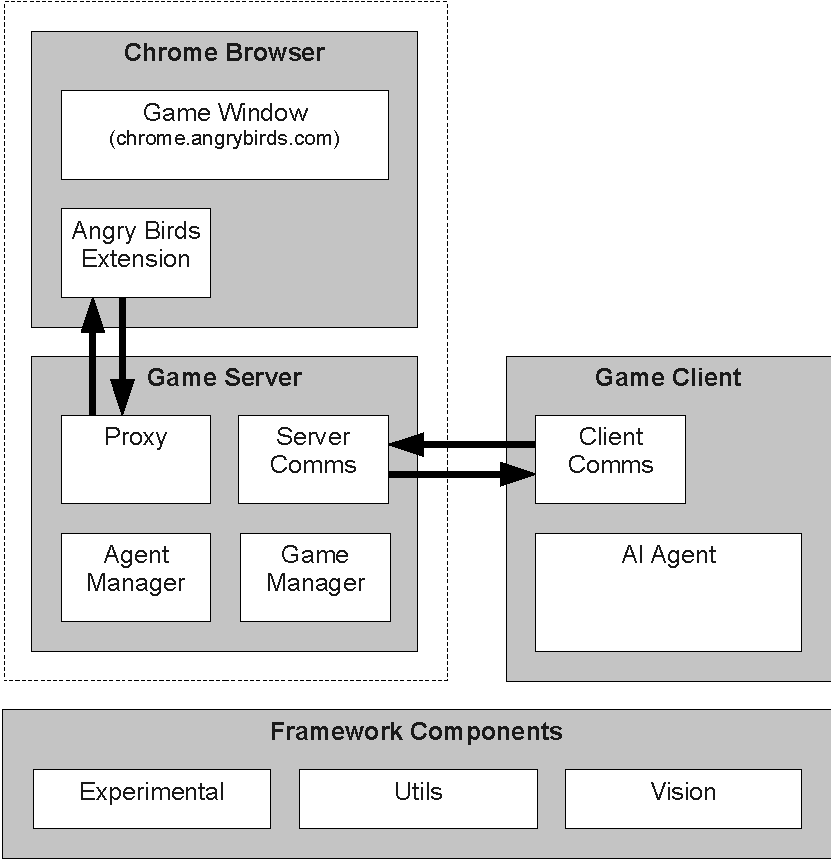
\includegraphics[width=0.5\textwidth]{archdiagram}
  \caption{Components of the AngryBirds AI Framework.}
\end{figure}

% Client/Server Messages --------------------------------------------------

\section{Client/Server Messages}
\label{sec:messages}

TODO: overview

\subsection{Login}

Client sends username and password. Server responds with OK (and list
of possible levels) or ERROR (and human readable message).

\subsection{GetScores}

Client requests scores. Server responds with list of all available
levels and the client's best score for that level.

\subsection{LoadLevel}

Client requests a level to play. Server resonds with OK or ERROR (and
a human readable message).

\subsection{GetState}

Client requests the game state. Server responds with the STATE (busy
playing, waiting for action, level failed, level completed), IMAGE (if
busy playing or waiting for action), and SCORE.

\subsection{DoAction}

Client sends an action or action sequence to perform. Server responds
with OK or ERROR (and human readable message).

An action consists of a shot (parameterized as angle and strength) and
optional tap after a time delay. An action sequence consists of one or
more actions separated by a time delay.

\end{document}

